% BEGIN GENERATED:coverage_figure
% generator: cdrt.report 1 (coverage_figure)
% inputs: results/labs/lab7/attempt4/functional_records.jsonl 00968fd19027; fixtures/out/parameters.json 2d3cdf7c84cb
% lock_root: 59af9d417b6025e385258c7484e2f9349269299ffc8db46b78d8fda049da0dca  campaign: campaign-004
% commit: 14a86e55f4ba59bde407e00829916370219d84a6
\begin{figure}[pos=tbp]
\centering
% generator: cdrt.report 1 (figures/coverage.tex); lock_root: 59af9d417b6025e385258c7484e2f9349269299ffc8db46b78d8fda049da0dca; commit: 14a86e55f4ba59bde407e00829916370219d84a6
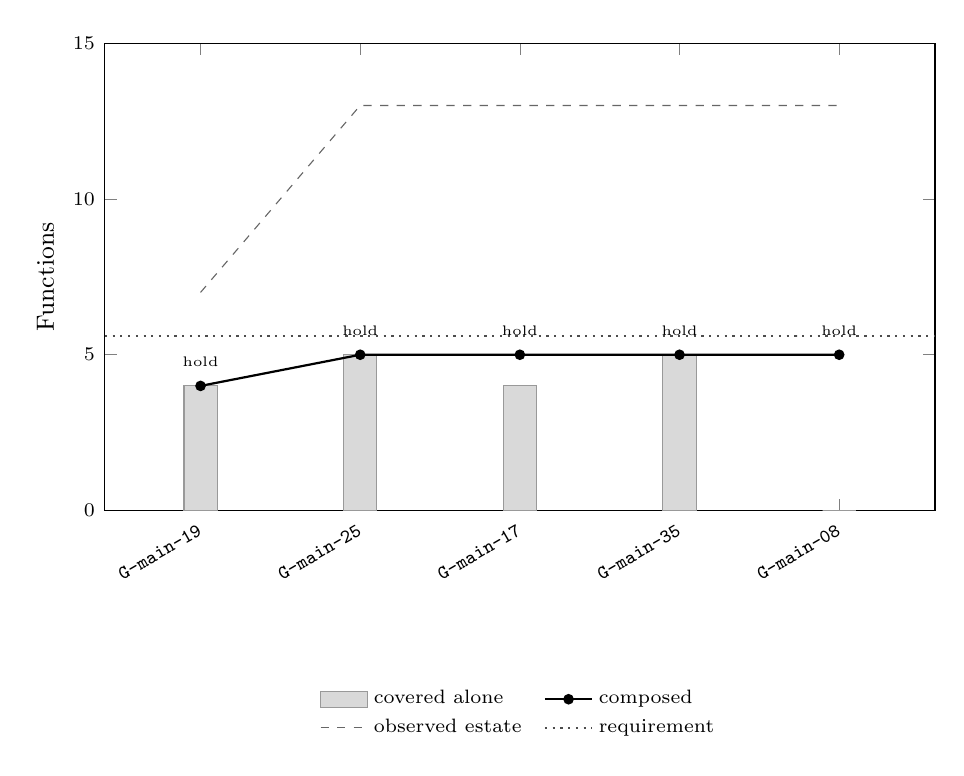
\begin{tikzpicture}
\begin{axis}[width=\columnwidth, height=0.62\columnwidth, ymin=0, ymax=15,
  xmin=0.4, xmax=5.6, xtick={1,2,3,4,5},
  xticklabels={{\texttt{G-main-19}},{\texttt{G-main-25}},{\texttt{G-main-17}},{\texttt{G-main-35}},{\texttt{G-main-08}}},
  xticklabel style={font=\scriptsize, rotate=30, anchor=north east}, ylabel={Functions},
  tick label style={font=\scriptsize}, label style={font=\small},
  legend style={font=\scriptsize, at={(0.5,-0.36)}, anchor=north, draw=none, fill=none, legend columns=2,
    /tikz/every even column/.append style={column sep=6pt}}, legend cell align=left]
\addplot[ybar, bar width=12pt, fill=black!15, draw=black!40, area legend] coordinates {(1,4) (2,5) (3,4) (4,5) (5,0)};
\addlegendentry{covered alone}
\addplot[thick, mark=*, mark size=1.5pt, black] coordinates {(1,4) (2,5) (3,5) (4,5) (5,5)};
\addlegendentry{composed}
\addplot[dashed, black!60, mark=none] coordinates {(1,7) (2,13) (3,13) (4,13) (5,13)};
\addlegendentry{observed estate}
\addplot[dotted, thick, black!70, domain=0.4:5.6] {5.6};
\addlegendentry{requirement}
\node[font=\tiny, anchor=south] at (axis cs:1,4.3) {hold};
\node[font=\tiny, anchor=south] at (axis cs:2,5.3) {hold};
\node[font=\tiny, anchor=south] at (axis cs:3,5.3) {hold};
\node[font=\tiny, anchor=south] at (axis cs:4,5.3) {hold};
\node[font=\tiny, anchor=south] at (axis cs:5,5.3) {hold};
\end{axis}
\end{tikzpicture}

\caption{Composed coverage as green decisions are admitted in capture order. Bars: release functions each decision covered on its own; solid line: release functions covered by all decisions admitted so far; dashed line: the size of the observed estate; dotted line: the requirement (\FixTauQ{} of \FixMq{}). The gateway reading after each admission is printed above. Only green decisions are shown; the 45 others are not eligible and do not change the composed coverage.}
\label{fig:coverage}
\end{figure}
% END GENERATED:coverage_figure
